\documentclass[12pt]{upenndiss}

% bibliography stuff
\usepackage{url}
\usepackage{natbib}
\bibpunct[:]{(}{)}{,}{a}{}{,}

% graphics
\usepackage{graphicx}

% tables
\usepackage{longtable}
\usepackage{multirow}
\usepackage{booktabs}

% my example environments
\usepackage{simplex}

% nice feature matrices
\usepackage{amsmath}

% (occasional) autosegmental diagrams
\usepackage{xypic}

% underlining in chap 2
\usepackage[normalem]{ulem}

% fonts
\usepackage{mathspec}
\setmainfont[Mapping=tex-text]{Linux Libertine}
\setmathfont(Digits,Greek,Latin){Linux Libertine}

%% KG's shortcuts
\newcommand{\buf}{\hspace{0pt}}
\newcommand{\gap}{\rule{1em}{0.5pt}}
\newcommand{\alt}{\ensuremath{\sim}}
\newcommand{\asp}{\textsuperscript{h}}
\newcommand{\pal}{\textsuperscript{j}}
\newcommand{\zero}{\ensuremath{\emptyset}}
\newcommand{\goesto}{\ensuremath{\longrightarrow}}
\providecommand{\e}[1]{\textsc{e}{$#1$}}

\title{Generative Phonotactics}
\author{Kyle Gorman}
\supervisor{Charles Yang \\ Associate Professor, Linguistics and Computer and Information Science}

\copyrighttrue

\department{Linguistics}

\abstractfile{abs} 
\acknowledgementsfile{ack}
\dedication{\center To my parents, Mark and Bev, who never once said *\emph{bnick} or *\emph{forwent}}

\begin{document}
\FrontMatter

\chapter{A program for phonotactic theory} \chapter{Sequence structure constraints in generative grammar}
\label{msc}

The first part of this text concerns the empirical substance of the theory of \textsc{Morpheme Structure Constraints} (MSCs), that is, language-specific constraints on the shapes of morphs stored in lexical memory.
Evidence is presented to support the claim that such constraints are solely derived by other components of grammar, and do not have an ontology of their own.

The first section of this chapter outlines a brief history of MSCs.
The following section draws upon this material to present the above claim as a null hypothesis, and presents conditions for falsifying it.
The final section outlines the remainder of Part I (chapters 2--4), which present evidence in support of this hypothesis.

% it is not clear what follows from a phonotactic description
% pater on NC
% can't be right tho, see stanley, kisseberth, clayton, shibatani, hooper, etc.

\section{A brief history of MSCs}

\subsection{Structuralism}

Since, with the possible exception of Roman Jakobson (who might be labeled an early generativist), the mentalistic interpretation of structural linguistic analyses was anathema, one must take care to not assume that a description of MSCs is something that these linguists would posit as part of speakers' knowledge of language.

\subsubsection{Morpheme boundaries in phonology}

bloomfield

%While \citeauthor{Bloomfield1930} is known for introducing morphemic structure into phonology, a member of the Prague circle developed an arguably more sophisticated approach only two years later. 

\citet{Jakobson1932} attributes a number of phonological properites of the Russian imperative to morpheme juncture. The vast majority of Russian infinitives consist of the stem followed by a theme vowel and /t\pal/. The reflexive is marked wih a final /-sə/ which feeds a general process of regressive voicing assimilation. In the reflexive infinitive, /\ldots t\pal-s\ldots/ is realized [ts], with no palatalization. However, palatalization of a stem-final labial or coronal---including /t\pal/, as in (\ref{russian}c)---is preserved in the reflexive imperative.

\begin{example}
\label{russian}
Russian reflexives \citep[after][]{Jakobson1932}:\footnote{I have taken a number of liberties with \citeauthor{Jakobson1932}'s presentation of the data, which uses an abstract phonemic transcription. Thanks to Lev Blumenfeld (p.c.) for help with the transcription of this data.}

\begin{tabular}{l l l l} %\toprule
   &  infinitive      & imperative \\ %\midrule
a. & [slav\pal itsə]  & [slaf\pal s\pal ə]  & `be glorious'    \\
   & [upram\pal itsə] & [upram\pal s\pal ə] & `be stubborn'    \\
b. & [kras\pal itsə]  & [kras\pal s\pal ə]  & `put on makeup'  \\
   & [ʒar\pal itsə]   & [ʒar\pal s\pal ə]   & `roast'          \\
c. & [zəbytsə]        & [zəbut\pal s\pal ə] & `forget' \\ %\bottomrule
%   & ab\'utsa      & ab\'ujsa     & `put on shoes'   \\
\end{tabular}
\end{example}

\noindent The forms in (\ref{russian}c) have different outcomes for their /t\pal-s/ clusters. \citeauthor{Jakobson1932} proposes that the preservation of palatalization is a special property of the imperative. %A few years later, \citet{Trnka1936}, another member of the Prague Circle, makes the connection between \citeauthor{Jakobson1932}'s hypothesis and phonotactic generalizations.

\subsubsection{The morph as a constraint domain}

A corrolary of this hypothesis is that the phoneme sequences found within morphs may be distinct from those which span multiple morphs. 

This was apparent to structuralists 

the phonologists 
This is apparent from 
a discussion of constraints on vowel sequences in Mixteco given by \citet{Pike1947b}.
It is apparent that \citeauthor{Pike1947b}'s constraints on vowel sequences are not intended to hold across morph boundaries, 

according to the phonological analysis of a Mixteco text published a few years earlier \citep{Pike1944}.

\begin{example}
Mixteco MSCs \citep{Pike1947b} and complex words \citep{Pike1944}:

\begin{tabular}{r l l l} %\toprule
   & MSC & complex exception \\ %\midrule
%a. & *{C}a{C}e & [k\'a-\textsuperscript{n}dee] & `kept \ldots inside' \\
%b. & *{C}\textipa{@}{C}e & [n\`i-k\`ə bə-de] & `who entered'        \\
%c. & *{C}e{C}i & [te-n\'i-ke\textsuperscript{n}da] & `was walking         \\
%d. & *{C}i{C}e & [te-n\`i-kee-t\`ə] & `and went away'      \\ %\toprule
%e. & *{C}e{C}o & b\'e\textglotstopvari e-\v{z}\'o & `our house'          \\
%f. & *{C}eo & ke-o-d\'e & `we eat him'         \\
a. & *{C}a{C}e & [ká\textsuperscript{n}dee] & `kept \ldots inside' \\
b. & *{C}ə{C}e & [nìk\`əbəde] & `who entered'        \\
c. & *{C}e{C}i & [teníke\textsuperscript{n}da] & `was walking         \\
d. & *{C}i{C}e & [tenìkeet\`ə] & `and went away'      \\ 
\end{tabular}
\end{example}

\noindent \citet[][166]{Pike1947b} affirms that the morpheme is ``marked'' by the violation of morpheme-internal sequence restrictions, an idea further developed by \citet{Harris1955} as a morpheme discovery routine.

\subsubsection{Biuniqueness and neutralization}

joos
harris
chomsky

\subsection{Early generativism}

\subsubsection{\citealt{Stanley1967}}

inventory constraints
sequence constraints

\subsubsection{Surface constraints and occultation}

shibatani
stampe
dell

\emph{A}[mt] `office', \emph{Anbau} `cultivation'
\emph{ei}[n.g]\emph{reifen} `to intervene',

\subsubsection{The duplication problem}

\citeauthor{Anderson1974} sees the duplication of \textsc{Backness Harmony} as both sequence structure constraint and phonological rule as a foregone conclusion
.The tendency of sequence structure constraints to duplicate phonological rules was noted by \citet[][401f.]{Stanley1967} and in \emph{SPE} (p.~382) in the discussion of morpheme structure constraints, and is labeled ``the duplication problem'' by \citet[][?]{Kenstowicz1977}.

inventory problems 
dell, chung, but also problems

conspiracies

\subsection{Autosegmentalism}

also ``supersegmentalism''

The proposals during this period are very diverse. 

\subsubsection{Syllable structure}

hooper
noske

\subsubsection{Morph features}

Leben
Kaye

\subsubsection{The Obligatory Contour Principle}

\subsection{Classic Optimality Theory}

%(page numbers here are taken from the published version)

\subsubsection{Richness of the Base}

some quotes from OT doc
\citet{PE}
\citet{Bye2001}

\subsubsection{Freedom of Analysis}

\citet{Smolensky1996}
\citet{PE}

\subsubsection{Undominated constraints}

% complaints about maceahern, gallagher
% bit on loanword adaptation

\subsection{Recent developments}

\subsubsection{Language acquisition}
% jusczyk forever
% white et al.
% early word learning
% syllables

\subsubsection{Psycholinguistic tasks in adults}

% wordlikeness
% spotting
% error correction, etc.

\subsubsection{Non-native word adaptation}

% perceptual factors

\section{The null hypothesis}

\subsection{The empirical proposal}

\subsection{The acquisition principle}

\subsection{Falsifiability}

%\subsection{Universal constraints?}    % 1.2.4: Universal constraints?
% This may be cut.

(see \citealt[][323f.]{Hockett1947}, \citealt[][415f.]{Nida1948}, \citealt[][50f.]{Anderson1992}, \citealt[][36f.]{Stump2001a}). Irrespective of one's position on this debate, it does not seem correct to extend this hypothesis to lexical roots. For instance, there  

imperfect subjunctive  & īrem     & īrēs     & īret     & īrēmus     & īrētis     & īrent \\
pluperfect subjunctive & issem    & issēs    & isset    & issēmus    & issētis    & issent \\
imperfect subjunctive  & venīrem  & venīrēs  & venīret  & venīrēmus  & venīrētis  & venīrent \\
pluperfect subjunctive & vēnissem & vēnissēs & vēnisset & vēnissēmus & vēnissētis & vēnissent \\

That this is not the 

While it might be possible to analyze \emph{ueni:re} as ``athematic'' /weni:-re/ and \emph{i:re} as /i:-re/, the frequentive \emph{uentita:re} `come often, be wont to come', formed with the \emph{-tit-} frequentive suffix (see \citet[][\S263]{Allen1903}), which selects for the first conjugation (cf.~\emph{agere} `act, make' vs. \emph{actita:re} `act, make often/repeatedly') suggests /wen-/.

It is also interesting to note that the same pattern has emerged in the history of French for a set of verbs which do not share this property in Latin. and the future and conditional indicative forms of \emph{aller} `go' and \emph{cuire} `to cook' in French.\footnote{\emph{Cuire}, interestingly, is not descended from the same conjugation as Latin \emph{i:re}, but rather from Latin \emph{coquere}; thus this syncretism is not simply an etymological relic of Latin. The same holds for other French verbs that inflect in the same manner, such as \emph{conduire} `drive (a vehicle); behave' and \emph{d\'etruire} `destroy'.}

future indicative      & irai   & iras   & ira      & irons    & irez    & iront \\
conditional indicative & irais  & irais  & irait    & irions   & iriez   & iraient \\
future indicative      & cuirai & cuiras  & cuira   & cuirons  & cuirez  & cuiront \\
conditional indicative & curias & cuirais & cuirait & cuirions & cuiriez & cuiront \\

One could even conceive of a largely vacuous principle on morpheme structure which simply requires that some subset of morphs not be null. 

%Anttila 2008
%Dmitrieva et al. 2008a,b
%Duanmu 2009
%Berkley 1994a,b, 2000
%Buckley 1997
%Coetzee 2008, Coetzee and Pater 2008
%Goad 2011
%Graff & Jaeger in press,
%Hammond 1999
%Colavin 2010,
%Frisch 1996, Frisch et al. 2004
%Hayes & Wilson 2008
%Kessler et al. 1997
%Martin 2007
%McGowan 2011
%Mester 1986
%Fudge 1969
%Padgett 1992
%Pierrehumbert 1993, 1994


\section{Outline of the dissertation}

%Chapter 2
%Chapter 3
%Chapter 4

\chapter{Categorical and gradient aspects of wordlikeness} \chapter{Categorical and gradient aspects of wordlikeness judgements} 
\label{gradience}

Two nonce words, \emph{blick} [blɪk] and \emph{bnick} [bnɪk], underlie the claim that speakers can rapidly distinguish between possible and impossible words \citet{Halle1962}. In \emph{SPE}, \citet{SPE} use a third word, \emph{bnzk}, to argue that nonce words fall on a cline of well-formedness. Neither \emph{bnick} nor \emph{bnzk} are possible words of English, they are possible words in other languages: stop-nasal onsets are found in Moroccan Arabic (e.g., \emph{bniqa} `closet') and stop-nasal-fricative-stop words in Imdlawn Tashlhiyt Berber \citep{Dell1985}. However, there is some sense in which \emph{bnzk} is even less English-like than \emph{bnick}. Of this, \citeauthor{SPE} write:

\begin{quote}
Hence, a real solution to the problem of ``admissibility'' will not simply define a tripartite categorization of occurring, accidental gap, and inadmissible, but will define the `degree of admissibility' of each potential lexical matrix in such a way as to\ldots{}make numerous other distinctions of this sort (\emph{SPE}:416--417)
\end{quote}

\noindent
The position that the well-formedness of nonce words is consistent the view of syntactic grammaticality taken in \emph{LSLT} and \emph{Aspects} \citep{LSLT,ASPECTS}, where it is claimed that different syntactic violations result in different degrees of ungrammaticality.

Most recent discussions of the ``problem of admissibility'' focus on this cline of wellformedness as it is evidenced in wordlikeness tasks.

\begin{quote}
When native speakers are asked to judge made-up (nonce) words, their intuitions are rarely all-or-nothing. In the usual case, novel items fall along a gradient cline of acceptability. \citep[][9]{Albright2009a}

In the particular domain of phonotactics gradient intuitions are pervasive: they have been found in every experiment that allowed participants to rate forms on a scale.
\citep[][382]{Hayes2008a}

\ldots{}when judgements are elicited in a controlled fashion from speakers, they always emerge as gradient, including all intermediate values. \citep[371]{Shademan2006} 
\end{quote}

\begin{quote}
\ldots{}A defect of current grammatical acounts of phonotactics is that they render simple up-or-down decisions concerning well-formedness and cannot account for gradient judgements. \citep[371]{Shademan2006}
\end{quote}

\citet[382]{Hayes2008a} ``consider the ability to model gradient intuitions to be an important criterion for evaluating phonotactic models''.

\begin{quote}
No integer seems to sit on the fence, undecided as to whether it is quite even, or perhaps a bit odd. No odd number seems odder than any other odd number. \citep[274]{Armstrong1983}
\end{quote}

\begin{quote}
Some have responded to these findings very consistently, by asserting that the experimental findings are to be interpreted as before: that, psychologically speaking, odd numbers as well as birds and vegetables are graded concepts\ldots{} We reject this conclusion just because we could not explain how a person could compute with integers who believed that 7 was odder than 23. We assert confidently that the facts about subjects being able to compute and about their being able to give the definition of odd number, etc., are the more important, highly entrenched, facts we want to preserve and explain\ldots{} we ourselves are prepared to give up the seeming fact that some odd numbers appear, as shown by their behavior in certain experimental paradigms, to be odder than others\ldots{}we do not give it up by saying that it was no fact; rather, by saying it must have been a fact about something other than the structure of concepts. \citep[284]{Armstrong1983}
\end{quote}

\begin{quote}
\ldots{}we hold that \emph{fruit} and \emph{odd number} have different structures, and yet we obtain the same experimental outcome for both. But if the same result is achieved regardless of the concept struture, then the experimental design is not pertinent to the determination of concept structure. \citep[284--5]{Armstrong1983}
\end{quote}

At first blush, this would seem to argue against a naïve account of wellformedness judgements in which ill-formedness results when prosodic parsing fails (e.g., \citealt{Ito1989a}, \citealt{Noske1992}, \citealt{OT}). Consider the possibility that a nonce word is ill-formed if it cannot be syllabified without modification. There is a long history for the proposal that impossible words are those whose surface form cannot be parsed into prosodic structures like syllables without further phonological modification (e.g., 

\begin{figure}
\centering
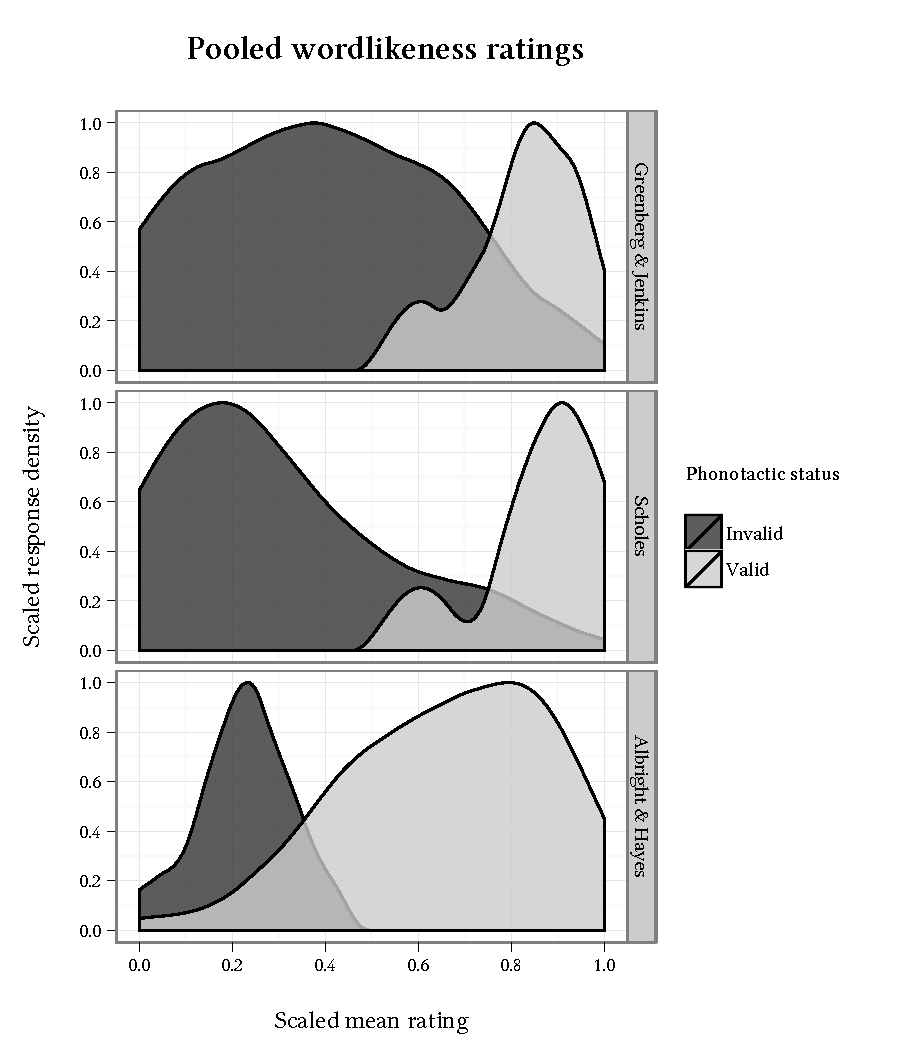
\includegraphics{density.pdf}
\caption{Average ratings of individual nonce words, linearly transformed to fit the interval [0, 1]}
\label{dsn}
\end{figure}

\begin{table}
\centering
\begin{tabular}{l rrr}
\toprule
                        & subjects & items & trials \\
\midrule
\citealt{Albright2007}  & 68       & 40    & 2,720  \\
\citealt{Albright2003a} & 24       & 87    & 2,064  \\
\citealt{Scholes1966}   & 33       & 63    & 2,178  \\
\midrule
\textsc{Total}          & 125      & 187   & 6,962  \\
\bottomrule
\end{tabular}
\caption{Subject and item counts}
\label{counts}
\end{table}

\begin{table}
\centering
\begin{tabular}{l rrrr}
\toprule
Pearson $r$               & \textsc{prosody} & \textsc{maxent} & \textsc{bigram} & \textsc{density} \\
\midrule
\citealt{Albright2007}    & \textbf{.725}    & {.703}          & {.463}          & {.695}           \\
\citealt{Albright2003b}   & {.594}           & {.208}          & \textbf{.746}   & {.688}           \\
\citealt{Scholes1966}     & {.803}           & {.534}          & {.737}          & \textbf{.834}    \\
\midrule
Spearman $\rho$           & \textsc{prosody} & \textsc{maxent} & \textsc{bigram} & \textsc{density} \\
\midrule
\citealt{Albright2007}    & \textbf{.819}    & {.661}          & {.338}          & {.612}           \\
\citealt{Albright2003b}   & {.662}           & {.389}          & {.699}          & \textbf{.739}    \\
\citealt{Scholes1966}     & {.769}           & {.575}          & {.794}          & \textbf{.817}    \\
\midrule
Kendall $\tau_{b}$        & \textsc{prosody} & \textsc{maxent} & \textsc{bigram} & \textsc{density} \\
\midrule
\citealt{Albright2007}    & {.666}           & \textbf{.683}   & {.245}          & {.450}           \\
\citealt{Albright2003b}   & {.474}           & {.159}          & {.499}          & \textbf{.558}    \\
\citealt{Scholes1966}     & {.619}           & {.484}          & {.614}          & \textbf{.671}    \\
\midrule
Goodman-Kruskal $\gamma$  & \textsc{prosody} & \textsc{maxent} & \textsc{bigram} & \textsc{density} \\
\midrule
\citealt{Albright2007}    & \textbf{.874}    & {.849}          & {.502}          & {.574}           \\
\citealt{Albright2003b}   & \textbf{.929}    & {.606}          & {.246}          & {.488}           \\
\citealt{Scholes1966}     & \textbf{.907}    & {.558}          & {.628}          & {.738}           \\
\bottomrule
\end{tabular}
\caption{FIXME}
\label{scores}
\end{table}

%\subsubsection{Maximum entropy phonotactics}
%
%\citeauthor{Hayes2008a} (\citeyear{Hayes2008a}; henceforth H\&W) develop a sophisticated model of phonotactic grammaticality which estimates a probability distribution over phoneme sequences by weighing constraints according to the principle of maximum entropy, following \citet{Goldwater2003} and \citet{Jager2007}. H\&W report that the predictions of their model are closely correlated with the \citet{Scholes1966} wordlikeness ratings. A direct replication of their predictions was attempted by using the software, model parameters, and training data as described in that study. Since the training of the maximum entropy model is inherently stochastic, producing slightly different outcomes on each run, the lowest scoring of ten runs is reported (H\&W:396), though in general there is not a great deal of variation between individual runs. One limitation of this model is that it is not feasible to score whole words, as the number of constraints which must be inspected grows exponentially as the span of possible constraints increases. Following H\&W and of \citet{Albright2009a}, who also applies the maximum entropy model to the \citet{Albright2003b} norms, the model is trained and scored only on stimulus onsets. However, as a consequence, the maximum entropy model performs particularly poorly on this data set, as many stimuli contain phonotactic violations in rime positions.
%
%\subsubsection{Segment bigram probability} 
%\label{bigram}
%
%The bigram probability of a sequence $ijk$ is the product of the probability of an sequence-initial $i$, the probability that $j$ follows $i$, and the probability that $k$ follows $j$, and the product of sequence-final \emph{k}.
%
%\begin{unlabeledexample}
%$\displaystyle \hat{p}(ijk) = p(i|\textrm{start}) \cdot p(j|i) \cdot p(k|j) \cdot p(\textrm{stop}|k)$
%\end{unlabeledexample}
%
%\noindent \citet{Albright2009a} employs bigram probability to model wordlikeness judgements. While the focus of \citeauthor{Albright2009a}'s study is on developing a model which uses bigrams over phonological features rather than segments themselves, \citeauthor{Albright2009a}'s evaluation, which includes both the \citeauthor{Scholes1966} and \citeauthor{Albright2003b} data sets, finds an advantage for segmental bigrams. \citeauthor{Albright2009a} does not provide an implementation of the featural bigram model, nor does his study describe it in sufficient detail to allow for a new implementation, but segmental bigram scores for the \citeauthor{Albright2003a} data are reported in the appendix. As reported by \citeauthor{Albright2009a}, segmental bigrams outperform featural bigrams (see Table \ref{albrightimproved}).
%
%\citeauthor{Albright2009a} estimates bigram probabilities using the method of maximum likelihood over types in the lexicon. The variant of segmental bigrams used here computes probabilities with a simple type of smoothing in which the count of all possible bigrams (including those never observed) are incremented by one. This technique is known as Laplace, or ``add one'' smoothing. This has the desirable effect that no nonce word is ever assigned a zero probability, and produces a small increase in the correlation between the \citeauthor{Albright2003b} wordlikeness norms compared with the maximum likelihood estimate (Table \ref{albrightimproved}). For all three data sets, this model also consistenly outperforms positional probability models defined by \citet{Vitevitch2004} and \citet{Vaden2009}; given that these model scores are highly correlatd with bigram probability \citep[][54]{Vitevitch1997}, they are not considered further. The bigram model consistently performs well in all the evaluations, and has the highest Spearman correlation with the \citeauthor{Greenberg1964} and \citeauthor{Scholes1966} data, and is frequently second place model to the binary baseline elsewhere.
%
%\subsubsection{Neighborhood density} 
%\label{density}
%
%There are now many methods for computing similarity between nonce words and existing words, long thought to be reflected in wordlikeness judgements. 
%For this study, a number of such methods were evaluated, including the Generalized Neighborhood Model \citep{Bailey2001}, PLD20 \citep{Suarez2011}, and a number of variations on neighborhood density \citep{Coltheart1977} provided by \citet{Vaden2009}. The best performance was obtained with the simplest version of neighborhood density, which is defined as the number of real monomorphemic words which can be changed into the target nonce word by a single insertion, deletion, or substitution of a phone.\footnote{\citet{Greenberg1964} use a variant in which only substitutions are counted.} For instance, the neighbors of \emph{blick} include \emph{blink} (insertion), \emph{lick} (deletion) and \emph{black} (substitution). While many studies \citep[e.g.,][]{Bailey2001} report robust lexical similarity effects, it may be that the relatively weak performance of neighborhood density is the result of the presence of gross phonotactic violations.
%
%\subsection{Modeling residual gradience}
%
%The primary result is that no gradient model reliably exceeds the accuracy of the binary baseline. Despite this, there are relatively strong correlations between the binary baseline and these gradient models (see Table \ref{bcor}). From the strong performance of the categorical model one can infer that the gradient models do not reliably predict intermediate ratings, or contrasts in ratings between words which are grouped together. To quantify this, the following method was used to estimate the residual contribution of the three gradient models once gross phonotactic violations are taken into account. Instead of calculating rank correlations directly on the model scores as in Table \ref{cor}, the model scores are mapped to ranks with the additional constraint that all ``valid'' stimuli be ranked above all ``invalid'' stimuli. The resulting ranks are used to compute new correlation statistics. Finally, the binary baseline correlation is subtracted from this number, so that the resulting value is the amount of improvement derived from augmenting the binary model with gradience. These difference numbers are shown in Table \ref{controlled}. In most cases, including the gradient models on top of the binary baseline produces a worse correlation than is obtained with the binary baseline alone.
%
%For $\tau_b$ and $\gamma$, the interpretation of this result is clear. The gradient models assign rankings to the sets of phonotactically valid and invalid clusters, respectively. For instance, the bigram model favors \emph{troog} [tɹuːɡ] over \emph{swach} [swætʃ], though neither contains any gross phonotactic violation. Similarly, the bigram model favors \emph{chwoop} [tʃwuːp] over \emph{zhrick} [ʒɹɪk], even though both contain ill-formed onsets. However, the majority of such predicted contrasts are not reflected in speakers' judgements; for instance, \emph{troog} is rated less English-like than \emph{swach} \citep{Greenberg1964}, contrary to the model predictions. This shows quite starkly that these models fail to reliably predict intermediate ratings.
%
%\subsection{The gradience hypothesis}
%
%This chapter has evaluated the axiom of gradience as a falsifiable alternative hypothesis. The surprising result is that virtually all of the apparent coverage of state-of-the-art gradient phonotactic models is simply a reflection of their ability to distinguish between the possible and the totally impossible; beyond this, they are unreliable. A trivial baseline, endowed with few abilities to project beyond the observed data, generally outperforms the state of the art. The projections made by the state-of-the-art gradient models are not like those made by speakers. It remains to be seen is whether any model can be put forth which accurately predicts these intermediate ratings.
%
%These result provide support for recent findings that speakers asked to perform gradient syntactic judgements produce responses closely corresponding to a widely recognized categorical grammatical/ungrammatical distinction \citep{Sprouse2007}.
%
%\subsection{Extensions to the binary baseline}
%
%The strong performance of the binary baseline should not be taken as evidence either that wordlikenesss judgements are binary, or that the binary baseline is a plausible model. The most serious limitation of this evaluation is the primitive nature of the binary baseline. The inability to generalization within onsets and rimes is a serious flaw, as is the assumption of independence of onset and rime. Regarding the rime, \citet{Borowsky1989} proposes a theory of possible rimes in English, which does make the correct prediction regarding the unattested but well-formed [ɛsp]. On the other hand, a cognitively plausible version of this model might need to entertain phonotactic generalizations that are larger than these units, since syllable-sized phonotactic generalizations have been proposed for English \citep[e.g.,][]{Berkley1994a,Berkley1994b,Coetzee2008b,Fudge1969}. 
%
%A possible further extension to the binary baseline would be the introduction of additional levels of wellformedness. While the evaluation has shown that current gradient models do not reliably identify intermediate wellformedness, it does seem possible to identify at least three levels of grammaticality: for instance, one might encode the intuition that \emph{zhlick} [ʒlɪk] is more English-like than \emph{bnick}, though both have unattested onsets. There are precedents for labeling certain attested words as phonotactically ``peripheral'' (see, e.g., the appendices in \citealt{Myers1987} and \citealt{Borowsky1989}); such words are regarded as lexical exceptions to language-general principles of syllabification. If this extends to nonce words, then an intermediate level of grammaticality could be assigned to ``possible'' but formally marked words. Another likely source of additional levels of grammaticality is the cumulative effect of multiple phonotactic violations. While, as \citet{Coleman1997} note, classical Optimality Theory predicts that a nonce word is as ill-formed as its worst deviation from syllable structure, it is possible to imagine that multiple phonotactic violations would result in greater degrees of ill-formedness. The bigram and maxent models make this prediction, as do many others \citep[e.g.,][]{Legendre1990,Levelt2000,Albright2008,Anttila2008a,Pater2009b} but despite this, there is still little data demonstrating cumulative effects in wordlikeness tasks.
%
%\subsection{Language acquisition}
%
%The weak empirical status of gradient phonotactic knowledge as reflected in adults has rammifications for language acquisition under the hypothesis that that infants acquiring language deploy the same representations as adults \citep[e.g.,][]{Macnamara1982,Pinker1984,Crain1991,Carey1995,deVilliers2001,Legate2007}. Gradient wordlikeness judgements in adults would provide support for claims that infants recognize statistical(inherently gradient) dependencies between segments \citep{Jusczyk1994} and use these to segment words \citep{Saffran1996}. An emerging consensus suggests, however, that infants attend to transitional probabilities primarily in the absence of grammatical cues \citep{Gambell2005,Hohne1994,Johnson2001,Jusczyk1999c,Lignos2012b,Mattys2001a,Shukla2007,Lew-Williams2012}. The vacuous nature of current evidence for gradient phonotactic knowledge in adults further weakens any hypothesis that would link statistical learning in infants to adults' behaviors.
%
%\section{Conclusion}
%
%%For instance, infants as young as 4.5 months seem to be aware that English nasal codas agree in place with following obstruents \citep{Mattys2001b,Jusczyk2002,Davidson2004}. 
%%It might be the case that syllable co-occurrence statistics might be little more than a reflection of infants' learning of categorical ``lexical viability'' constraints \citep{Johnson2003} of the sort also seen in adult speech processing \citep[e.g.,][]{Norris1997}. 
%
%% other ratings, but por qué?:
%% 
%% Hayes2000
%% 
%% Albright2003a
%% Albright2003b
%% Prasada1993 
%% 
%% Bard1996
%% 
%% Koo2009
%% 
%% Treiman2000
%% 
%% Warker2006
%% 
%% Massaro1983
%% 
%% Rusaw2009
%do not explicitly state why this data is relevant to the construction of models of wordlikeness. Presumably, these authors believe that these patterns of judgements demonstrate that wordlikeness, as an internal state, is gradient simply because subjects make use of intermediate degrees of wordlikeness in judgement tasks. This proposition, generalized below, is ``naïve'' not because it lacks sophistication, but because it is rooted in a belief in naïve realism, a philosophy which holds that perception provides a relatively direct picture of the nature of the world, an influential view in the cognitive sciences in general (see \citealt{Fodor1981a} for a critique).
%
%\citeauthor{Chomsky1965} were not the first to consider the notion of possible and impossible words. Their primary contribution is that their mentalist perspective: they recognize that naïve speakers effortlessly acquire language-specific generalizations about possible and impossible words and can report them without any explicit training.
%
%However, not all early literature is concerned with gradience. \citet[31]{Vogt1954}, for instance, recognizes that the taxonomic phoneme is insufficient to account for many wordlikeness contrasts. \citeauthor{Vogt1954} observes that allophony may account for the absence of certain phone sequences, but it does not provide a suitable explanation for the absence of initial [bn] in English, nor does it make correct predictions about the surface realization of an underlying initial /bn/. \citeauthor{Vogt1954} concludes that additional grammatical machinery will be needed to account for possible and impossible words. 
%
%Most relevant to the question at hand, \citet{Frisch2000} and \citet{Vitevitch1997} find that speakers' wordlikeness ratings of multisyllabic words are correlated wtih the positional probailities of the constituent syllables. Unfortunately, none of these researchers make any effort to eliminate the possibility that the low positional probability stimuli are ``impossible'' words of English. In fact, 
%Chapter \ref{clusters} argues
%%the author has argued elsewhere \citep{Gorman2012c}
%that many of the stimuli used by \citeauthor{Frisch2000} and \citeauthor{Vitevitch1997} contain illicit word-medial consonant clusters. While \citeauthor{Vitevitch1997} neither control nor manipulate the well-formedness of medial clusters, in a post-hoc test they consider a probabilistic measure of cluster well-formedness, which reveals that cluster well-formedness is correlated with syllable-internal positional probabilities and wordlikeness judgements, but \citeauthor{Vitevitch1997} ultimately conclude this cannot explain all the variation in wordlikeness. 
%
%Using the head-term preference paradigm, \citet{Jusczyk1993b} and \citet{Friederici1993} find that typically-developing children as young as 9 months of age distinguish between nonce words which are and are not phonotactically valid in their target language. \citet{Jusczyk1994} report that 9-month-old children acquiring English also show preferences for nonce words with high positional probability over those with low positional probability. Faciliatory effects of positional probability (i.e., shorter latencies) are reported for other nonce word tasks conducted with adults, including single-word shadowing \citep{Vitevitch1997,Vitevitch1998}, same/different judgements \citep{Vitevitch1999a,Luce2001,Lipinski2005,Vitevitch2005}, and lexical decision \citep{Pylkkanen2002a}.
%
%The aforementioned studies all conclude that the gradient measure of positional probability correlates with behavioral results. As the flaws of the \citet{Vitevitch1997} study demonstrate, the aforementioned studies do little to tease apart the gradient and categorical aspects of phonotactics. More generally, they do little to distinguish between positional probability and closely correlated measures like bigram probability (see \S\ref{bigram} below) or neighborhood density, since these studies carefully select stimuli which either have high or low values for all of positional probability, bigram probablility, and neighborhood density. This is particularly troublesome given that no justification has ever been given for the positional probability measure in the first place; it appears to have been created \emph{ex nihilo}; in contrast, the effects of neighborhood density in various psycholinguistic tasks are emergent properties of many models of speech production \citep[e.g.,][]{Luce1998,Luce2000} and perception \citep{Marslen-Wilson1984,Marslen-Wilson1987,McClelland1986,Norris1994,Norris2000}. 
%\subsubsection{\citealt{Greenberg1964}}
%
%\citet{Greenberg1964} investigated wordlikeness using the technique of free magnitude estimation, a mechanism which has become increasingly popular among syntacticians \citep[e.g.,][]{Bard1996}. At the beginning of the experiment, the subject heard a recording of the word \emph{stick}. In subsequent trials, the subjects heard a nonce word and were asked to report ``how far would you say that is from English?'', with \emph{stick} at ``1''; subjects are told that a word that is ``twice as far from English'' as \emph{stick} should be scored ``2''. The data used here are from \citeauthor{Greenberg1964}'s Experiment B, in which 17 undergraduates were presented 17 stimuli in all. In addition to \emph{stick}, the stimuli include three other English words; these four items were excluded from further analyses, leaving 13 stimuli. As is standard practice in psychophysics \citep[e.g.,][]{Butler1987}, magnitudes were log-transformed prior to analysis.
%

\chapter{Static and derived Turkish phonotactics} \chapter{Static and derived constraints in Turkish}
\label{turkish}

glossematics

\citet{Chomsky1965} propose


In retrospect, it seems somewhat odd that \citeauthor{Chomsky1965} would coh
It might 
In defining the 

The contrast between \emph{blick} and \emph{bnick} is what has been called a "projection problem" \citep{Baker1979}

This is not a universal, but rather something English speakers must learn, as some languages, such as Moroccan Arabic, do in fact permit \emph{bn} onsets (e.g., \emph{bni} 'building', \emph{bnat} 'daughters', \emph{bniqa} 'closet'); 


\citet{Lees1966b,Lees1966a}


This is what we might call a projec
In presenting the components of a 
a term which 

by subphonemic details

\citet{Davidson2005,Davidson2006a} shows that excresent schwa is acoustically and articulatorily distinct from "lexical schwa":
\citet{Wilson2011} show taht speakers use this 

%English speakers' z^@k is more similar to \emph{scum} than \emph{succumb}

/sC-/ onsets than /s@C-/.

% Davidson 2005: z^@C is more like sC than s@C (ultrasound of articulations)
% Davidson 2006a: lexical and excresant schwa are not the same (acoustics)

% Davidson 2010: production
% Wilson & Davidson 2011:

\citet{Berent2007a}
\citet{Berent2007b}
\citet{Berent2008a}

% Berent et al. 2007
% 598: Highly marked inputs are repaired in perception to abide by the grammatical restrictions of the language
% Exps 1-2: syllable count task (misperception due to linguistic experience; "disyllables were more likely to be perceived as monosyllables if their monosyllabic counterparts had a less marked cluster" in both Russian and English, not what OT predicts)
% Exps 3-4: AB task
% Exps 5-6: priming effect (non-epenthetic and epenethetic things represented the same)
% Berent and Lennertz 2007: (640: If the high rate of monosyllabic errors to unmarked onsets is only due to phonetic failures to encode the input, then it is puzzling why the same onsets also yield the highest rate of accurate response.)
% Berent et al. 2008a:
\citet{Peperkamp2007}
% Peperkamp 2007: during one stage of processing phonology is undone with help from the lexicon...it only takes licit inputs and is irrelevant (p. 633)
\citet{Dupoux1999}
% Dupoux et al. 1999: Japanese speakers still can't distinguish between ebzo and ebuzo in an ABX task using the SAME a or b.


does not so much as explain the thing itself but rather suggests the

I believe a number of the predictions of this model are wrong
the original and still-compelling 
findings that drove 

 motivations for the development of a theory of static co-occurrence restrictions as developed by \citet{SPR}, \citet{Stanley1967} and others is to account for speakers' abilities to distinguish between accidental and structural gaps. \citet{Chomsky1965} propose that a theory of phonology must account for speakers' abilities to distinguish between accidental and structural gaps in their language, citing a contrast between \emph{blick}, which is judged to be a possible but unattested word of English, and \emph{bnick}, which is judged to be impossible. \emph{SPE} (p.~3810f.) places this contrast in a system of a system of sequence structure rules that also are used to eliminate lexical redundancy. In the phonological theory of the era, there is no process that could generate the \emph{blick} $\sim$ \emph{bnick} contrast or numerous other lexical regularities \citep[][283f.]{Anderson1974}.

This sequence of arguments has already been critiqued in Chapter \ref{1}, where it was shown that prosodic licensing and Stampean occultation places this contrast in core phonology, and that the principles by which speakers recognize impossible words must be stated on surface representations, not underlying representations. Further, \citet[][528f.]{Halle1975} rejects his own principle that lexical entries should be free of all redundancies (see \citealt[][201]{Reiss2003a} and \citealt{Vaux2003} for further discussion). This rejected principle of a redundancy-free lexicon is one of the two principles that motivates Morpheme Structure Constraints; the other is the subject of this and the following chapter.

the other being the subject 


a principle which is one of the two motivations  motivated the introduction of morpheme structure constraints.

In the preceding chapter, it was shown that apparent underrepresentation of certain sequences in the lexicon does not always require static constraints on possible underlying representations, since such distributions arise by chance and static constraints defined over natural classes contribute little to predicting the contents of the lexicon. 
%This result does not directly bear on the question of whether static restrictions have any synchronic reality.

Yet countless static constraints are statistically supported. Under the null hypothesis advanced in Chapter \ref{MSCs}, the lexical statistics of co-occurrence restrictions are irrelevant: the language acquisition device only attends to derived restrictions and ignores static restrictions regardless of their statistical reliability. On the other hand, many linguists assume that statistical significance provides sufficient conditions for positing synchronically active static constraints. For instance, \citet{Brown2010} writes:

\begin{quotation}
\ldots the patterns outlined above are statististically significant. Given this, it stands that these sound patterns should be explained by some linguistic mechanism. \citep[][48]{Brown2010}
\end{quotation}

\noindent
A nuanced version of this alternative hypothesis would recognize that there may be other necessary conditions. Any explicit theory of static constraints will have to impose formal restrictions on possible co-occurrence restrictions. The set of possible constraints must respect results in formal learning theory, and may also be, for example, constrained by naturalness biases or formal markedness considerations. 

A further widespread assumption is that static co-occurrence restrictions validated statistically will be reflected by wordlikeness judgements. This assumption is so deeply entrenched that a number of recent studies of phonotactic learning forgo wordlikeness judgements altogether and instead model the lexical statistics themselves (e.g., \citealt{Coetzee2008a} and \citealt{Anttila2008} on Muna and Arabic, \citealt[][385]{Hayes2008a} on Shona and Wargamay, \citealt{Brown2010} on Gitksan). 

Since the null hypothesis does not countenance statistical significance as evidence for the synchronic reality of a static lexical pattern, such patterns do not adjudicate between the null hypothesis and the alternative, and another source of evidence is needed. In the remainder of Part I, I turn to data from wordlikeness judgement tasks for these purposes. 

In a wordlikeness task, a speaker is presented with nonce words and asked to report such intuitions about the ``possibility'' of a word. 



The alternative hypothesis, then, is that a statistically reliable co-occurrence restriction will be reflected in native speakers' wordlikeness judgements. 

The data below, drawn from Turkish, shows that 



This chapter takes the argument one step farther by showing a contrast between static and derived constraints on URs in Turkish. Whereas the derived constraint has a robust effect on native speakers' wordlikeness judgements, the static constraint, which is equally statistically valid, has no effect on these judgements. Anticipating the conclusion, the simplest explanation for the non-effect of this static constraint on wordlikeness judgements is that speakers do not internalize static co-occurrence restrictions at all. 

%Classical Arabic adjectives often have stative verbs in which the root is imposed onto the template CaCuCa: 

%It is important to note that the nature of the \emph{blick}/\emph{bnick} contrast is no longer a mystery. 
%Generative phonological theory at the time of \emph{SPE} lacked the representational vocabulary to directly distinguish between word-initial /bn/, which is disallowed, and /bn/ as a licit syllable contact cluster (e.g., \emph{o}[b.n]\emph{oxious}), a point first made by \citep{Hooper1973}. It is not the introduction of prosodic primitives into generative phonology that explains the contrast between \emph{blick} and \emph{bnick}, though, but rather the principle that surface forms must be syllabified \citep[e.g.,][63f.]{Kiparsky1982b} which \emph{bnick} fails. If, as is standardly assumed, phonology repairs unsyllabifiable outputs \citep[e.g.][]{Ito1989a,Noske1992}, then \emph{bnick} is an impossible output, doomed to be modified (perhaps to \emph{nick}; \citealt[][19f.]{Wolf2009}), and /bnɪk/ is an impossible UR by Stampean occultation. 

\section{Turkish vowel MSCs}

\citet{Zimmer1969}

I assume without discussion the following binary feature specifications for the vowel phonemes of Turkish.

\ex Turkish vowel features: \vspace{6pt} \\
\begin{tabular}{c | c c c c}
                       & \multicolumn{2}{c}{[$-$\textsc{Back}]} & \multicolumn{2}{c}{[$+$\textsc{Back}]} \\
                       & [$-$\textsc{Round}] & [$+$\textsc{Round}] & [$-$\textsc{Round}] & [$+$\textsc{Round}] \\ \midrule
\buf[$+$\textsc{High}] & i & ü [y] & ı [ɯ] & u \\
\buf[$-$\textsc{High}] & e & ö [ø] & a [ɑ] & o \\
\end{tabular}
\xe

%\citep[][289]{Anderson1975}
%\citep{Clements1982}
%\citet{Inkelas1997}
%\citet{Harrison2001}

\subsection{Backness harmony}

One of the most salient properties of Turkish is its harmony system, which \citeauthor{Lees1966b} (\citeyear[][35]{Lees1966b}, \citeyear[][284]{Lees1966a}) derives by means of feature spreading rules. Backness harmony is the the most general of these processes.

\subsubsection{Phonological description}

The rule of \textsc{Backness Harmony} spreads a vowel's \textsc{Back} specification rightward over any intervening consonants onto the next vowel.  

%\citep[after][229]{Clements1982}: \\
\begin{example}
\textsc{Backness Harmony}:

\xymatrix@R=24pt@C=24pt{
\txt{V}                                        & \txt{C$_0$} & \txt{V} \\
\txt{[α \textsc{Back}]}\ar@{-}[u]\ar@{--}[urr] \\
}
\end{example}

This rule accounts for a great deal of the suffix allomorphy found in Turkish. For instance, the nominative plural (nom.pl.) suffix is \emph{-ler} when the final root vowel is [$-$\textsc{Back}], and \emph{-lar} when it is [$+$\textsc{Back}], as predicted by Backness Harmony.

\begin{example}
\label{turknom}
The Turkish nominative:

\vspace{0.5\baselineskip}
\begin{tabular}{l l l l l}
   & \emph{nom.sg.} & \emph{nom.pl.} \\
a. & ip             & ipler          & `rope' & \citep[][216]{Clements1982} \\
   & el             & eller          & `hand'    \\
   & köy            & köyler         & `village' \\
   & yüz            & yüzler         & `face'    \\
   & kız            & kizlar         & `girl'    \\
   & sap            & saplar         & `stalk'   \\
   & son            & sonlar         & `end'     \\
   & pul            & pullar         & `stamp'   \\
b. & neden          & nedenler       & `reason'  & (TELL) \\
   & boğaz          & boğazlar       & `throat'  \\
   & kiler          & kilerler       & `pantry'  \\
   & pelür          & pelürler       & `tissue paper' \\
   & sapık          & sapıklar       & `pervert' \\
\end{tabular}
\end{example}

There are a few complications, however. First, not all polysyllabic roots conform to \textsc{Backness Harmony}. In this case, as can be seen from (\ref{turkexcept}a), suffix vowels generally harmonize with the final root vowel. There is also a small class of nouns, shown in (\ref{turkexcept}b), which exhibit [$-$\textsc{Back}] suffix vowels despite the fact that their final root vowel is [$+$\textsc{Back}].

\begin{example}
\label{turkexcept}
Exceptional Turkish nominatives:

\vspace{0.5\baselineskip}
\begin{tabular}{l l l l l}
   & \emph{nom.sg.} & \emph{nom.pl.} \\
a. & mezar          & mezarlar       & `grave' & \citep{TELL} \\
   & model          & modeller       & `model' \\
   & silah          & silahlar       & `weapon'     \\
   & memur          & memurlar       & `bureaucrat' \\
   & sabun          & sabunlar       & `soap'       \\
b. & saat           & saatler        & `hour, clock' \\
   & harf           & harfler        & `(alphabetic) letter' \\ %& \citep{Goksel2005}
   & etol           & etoller        & `fur stole' \\
\end{tabular}
\end{example}

It is uncontroversial that the disharmonic suffixes of (\ref{turkexcept}b) are no more than very sporadic exceptions to \textsc{Backness Harmony}, root disharmony has ben the subject of much debate. As disharmonic roots still trigger suffix harmony, \citet[][212, 289]{Anderson1974} proposes to distinguish suffix harmony (an alternation) from a sequence structure constraint governing root harmony. This point is echoed by \citet{Iverson1978}.

However, as \citet[][197f.]{Zonneveld1978} notes, the theory of exceptionality proposed in \emph{SPE} (p.~374f.) provides a direct account of suffix harmony in disharmonic roots. \citeauthor{SPE} assume that the specification of the target (i.e., the segment or segments to be changed) of a rule $R$ must be marked [$+$rule $R$] by convention. A root or affix which fails to undergo $R$ despite otherwise matching the structural description is simply said to be marked [$-$rule $R$]. Under this account, exceptionality boils down to failing to match an extended structural description. If disharmonic roots are marked [$-$\textsc{Backness Harmony}], then the final vowel of disharmonic roots will still trigger \textsc{Backness Harmony}, since the [$-$\textsc{Backness Harmony}] root is no longer the target but rather the environment, which is not subject to the [$+$\textsc{Backness Harmony}] requirement.

%Once additional source of evidence on root (dis)harmony is inconclusive. There is a small class of bisyllabic words in which the second vowel, always [$+$\textsc{High}, $-$\textsc{Back}], alternates with zero. 

%\ex High-vowel/zero alternations \citep[][243]{Clements1982}: \\
%\begin{tabular}{l l l l}
%   & nom.sg. & gen.sg. \\
%a. & fikir   & fikri  & `idea' \\
%   & hüküm   & hükmün & `judgement' \\
%%  & filim   & filmi & `film' & \citep[][178]{Inkelas2001} \\
%b. & vakit   & vaktin & `time' \\
%   & rahim   & rahmin & `womb' \\
%\end{tabular} \xe
%
%\noindent
%It is possible that \textsc{Backness Harmony} might produce a fluctuating \emph{ı} after root \emph{a}, but this does not obtain (\lastx b). However, this might simply indicate that the fluctuating vowel is epenthetic and that harmony applies before epenthesis (see \citealt{Clements1982} for both sides of this argument), making it less than a counterexample. 

An alternative account, first proposed by \citet{Clements1982}, uses underspecificatio to derive the non-exceptionality of harmonic roots. The initial-syllable vowel of a Turkish root is contrastively specified for backness (e.g., \emph{kül} `ash' vs.  \emph{kul} `servant', \emph{kepek} `bran' vs. \emph{kapak} `lid'); harmonic roots are ones in which non-initial syllable vowels cannot contrast for this feature, and \citeauthor{Clements1982} proposes to leave them underspecified. Only in disharmonic roots does \textsc{Back} need to be specified for non-initial syllable vowels. 
%This is exemplified below in (\ref{spec}).
%(e.g., \emph{deve} `camel' vs. \emph{deva} `medicine', \emph{sene} `year' vs. \emph{sena} `praise'). 

%There is some further evidence that individual vowels may differ in specification for this feature even within individual roots or affixes. For instance, the present continuous suffix has harmony-determined allomorphs \emph{-iyor}, \emph{-üyor}, \emph{-ıyor}, \emph{-uyor}, but the \emph{o} of the suffix is invariant. A similar situation might obtain in Turkish roots. 

\begin{example}
\label{spec}
\textsc{Back} specification for (dis)harmonic roots: 

\vspace{0.5\baselineskip}
\xymatrix@R=24pt@C=24pt{
\txt{a.} & \txt{harmonic root:~~~~} & \txt{C} & \txt{V} & \txt{C} & \txt{V} \\
&   &    & \txt{[$-$\textsc{Back}]}\ar@{-}[u]\ar@{--}[urr] \\
\txt{b.} & \txt{disharmonic root:} & \txt{C} & \txt{V} & \txt{C} & \txt{V} \\
    &    &         & \txt{[$-$\textsc{Back}]}\ar@{-}[u] & & \txt{[$+$\textsc{Back}]}\ar@{-}[u]
}
\end{example}

\noindent
Harmonizing suffix vowels will also be underspecified for \textsc{Back}. Of course, \textsc{Backness Harmony} needs to be prevented from overwriting the [$+$\textsc{Back}] specification of disharmonic roots, one option being the use of a a \textsc{Structure Preservation} condition \citep{Kiparsky1985}. Unfortunately, this detail reintroduces the duplication alluded to above. Any condition on the rule of \textsc{Backness Harmony} which prevents overwriting entails that it has no control over the distribution of harmonic and disharmonic roots, and thus fails to account for predominance of harmonic roots.

\citet{Clements1982} and \citet{Kaun1999}

\footnote{Thanks to Kie Zuraw for bringing this data to my attention.}

the epenthetic vowel is always [$+$\textsc{High}], and when the first consonant of the cluster is non-dorsal, it shows backness harmony

\begin{example}
Adaptation of initial foreign clusters \citep[][247]{Clements1982}: 

\vspace{0.5\baselineskip}
\begin{tabular}{l l l l l l}
a. & spiker  & \alt{} & sipiker  & `announcer' \\
   & fren    & \alt{} & firen    & `break'     \\
   & trablus & \alt{} & tırablus & `Tripoli'   \\
   & brom    & \alt{} & burom    & `bromide'   \\
   & prusya  & \alt{} & purusya  & `Prussia'   \\
b. & kral    & \alt{} & kıral    & `king'      \\
   & grup    & \alt{} & gurup    & `group'     \\
c. & grip    & \alt{} & gırip    & `grippe'    \\ % unexpectedly back
   & kredi   & \alt{} & kıredi   & `credit'    \\
\end{tabular}
\end{example}

\subsubsection{Psycholinguistic evidence}

The evidence from alternations leaves open the question of whether speakers internalize a generalization regarding the tendency of roots to conform to \textsc{Backness Harmony}. One piece of evidence that speaks in favor of root-internal harmony comes from a language game discussed by \citet{Harrison2001}.\footnote{Thanks to Bert Vaux for bringing this study to my attention.} This game is not indigenous to Turkish, but it corresponds to a morphological process native to the related language Tuvan, in which it conveys a sense of ``vagueness or jocularity'', and \citeauthor{Harrison2001} report that it can be quickly taught to even young Turkish speakers. The game consists of reduplication of the base and replacement of the first vowel in the reduplicant with \emph{a} or \emph{u}. 

In both Tuvan and Turkish, the unchanged reduplicant vowel is also affected. Reduplication interacts with root harmony in both Tuvan and Turkish. When the base is harmonically [$-$\textsc{Back}], the insertion of a [$+$\textsc{Back}] results in what \citeauthor{Harrison2001} call ``reharmonization'' (\ref{redupgame}a).

\begin{example}
\label{redupgame}
Turkish reduplication game \citep[][231]{Harrison2001}:

\vspace{0.5\baselineskip}
\begin{tabular}{l l l l}
a. & kibrit & kibrit-kabrıt & `match'    \\
   & bütün  & bütün-batın   & `whole'    \\
b. & mali   & mali-muli     & `Mali'     \\
   & butik  & butik-batik   & `boutique' \\
\end{tabular}
\end{example}

\noindent
Under the underspecification hypothesis, non-initial harmonic vowels lack an underlying \textsc{Back} feature, so it comes as no surprise that changing the \textsc{Back} specification of the root-initial vowel results in reharmonization. And the full specification of disharmonic roots correctly predicts that they will be exempt from reharmonization (\ref{redupgame}b), which is also borne out in Tuvan and in an unrelated Finnish language game \citep{Campbell1986}.

A number of studies have found that speakers of Finnish use disharmony in speech processing experiments.\footnote{Thanks to Charles Yang for pointing out the relevance of these studies to me.} \citet{Suomi1997} and \citet{Vroomen1998} generate nonce trisyllabic words by adding a monosyllabic pseudo-prefix to real and nonce disyllabic words, all of which are harmonic for the feature \textsc{Back}. These stimuli are auditorily presented to subjects who are asked to press a button when the nonce trisyllable ends with a target nonce disyllable, or a real disyllabic word. Speakers are quicker to press the button when the prefix and disyllabic word disagree for \textsc{Back}. These results suggest that speakers are attuned to the fact that disharmonic transisitions are good predictors of word boundaries. If speakers have also internalized the converse generalization, that harmonic transistions are more likely to be root-internal, then there is additional evidence that harmony is active not just in Finnish affix alternations but also in roots. 

\citet{Kabak2010} report that Turkish \textsc{Backness Harmony} has the same effect on word-spotting as it does in Finnish: speakers are quicker and more accurate at the task of spotting the nonce target word \emph{pavo} when preceded by the pseudo-prefix \emph{gölü-}, a disharmonic transistion, than when it is preceded by the pseudo-prefix \emph{golu-}, a harmonic transition. \citeauthor{Kabak2010} find that effect of harmony does not obtain for speakers of French, a language which lacks vowel harmony. As in Finnish, the results imply speakers have internalized the predominance of root-internal harmony.

It seems that the root-internal harmony bias is in fact learned by Turkish speakers very early. The pseudoword spotting experiment has been adapted for 9-month-old Turkish infants by \citet{Kampen2008}. Infants are familiarized with harmonic disyllabic pseudowords bearing a pseudo-prefix, which may be harmonic or disharmonic. At test time, the infants are played the disyllabic pseudowords in isolation using the head turn preference paradigm. Infants show a preference to listen to those pseudowords which were familiarized with a disharmonic pseudo-prefix over those which were familiarized with a harmonic pseudo-prefix. This preference is not observed in 9-month-old infants learning German, which also lacks vowel harmony. Similarly, \citeauthor{Kampen2008} report that Turkish 6-month-old infants prefer to listen to harmonic pseudowords such as \emph{paroz} over disharmonic pseudowords like \emph{nelok}, but German 6-month-old infants show no such preference.

% 3.1.2: Lexical statistics

This is essentially the hypothesis pursued in the previous chapter.

\citet{TELL}
\citet{Inkelas2001}

%We might, for instance, consider methods based not on statistical \citep{Yang2005,Gorman2011b}.


\section{Evaluation}

The results reveal a dissociation between the lexical statistics and wordlikeness judgements, a dissociation that finds a natural explanation from the principle of ...

There is some disagreement in the literature about just what \citet{Zimmer1969} finds regarding \textsc{Backness Harmony} and \textsc{Labial Attraction}.

\subsection{Lexical statistics}

This choice of statistical test is justified in Section \ref{stattech}.

\subsubsection{Backness harmony}

\subsubsection{Roundness harmony}

%\ex Lexical effects of \textsc{Roundness Harmony} \citep{TELL}: \vspace{6pt} \\
%\begin{tabular}{l r r r r r}
%\toprule              & 
%Corpus                & $p$-value \\
%\midrule
%Full TELL             &  
%Elicited TELL         & 
%TELL with etymologies & 
%\end{tabular}
%\xe

%\citet{Harrison2004} 73\% 
%of lexical types are harmonic (both back and round)

\subsubsection{Labial attraction}

\begin{quotation}
Vowel labialization following labials is not a synchronic alternation in Turkish, yet it (unlike \textsc{Labial Attraction} per se) \emph{is} a statistically supported tendency worthy of further research. \citep[][196, emphasis in original]{Inkelas2001} 
\end{quotation}

%\ex Lexical effects of \textsc{Labial Attraction} \citep[][186]{Inkelas2001}: \vspace{6pt} \\
%\begin{tabular}{l r r r r r}
%\toprule
%Corpus                & aPu & aPı & aTu & aTı   & $p$-value   \\ % & corpus size
%\midrule
%Full TELL             & 378 & 248 & 446 & 1,140 & 2.83\e{-44} \\ % & 31,236 \\
%Elicited TELL         & 152 & 265 & 101 & 1,839 & 9.84\e{-60} \\ % & 16,541 \\
%TELL with etymologies & 128 & 109 &  79 &   470 & 6.56\e{-32} \\ 
%\bottomrule
%\end{tabular}
%\xe

%Etymological subset of TELL
%Native    & Foreign   \\
%aBu & aBI & aBu & aBI \\
%12  & 11  & 84  & 28  \\
%p = 0.0417

\subsection{Wordlikeness results}

There is some disagreement in the literature about just what \citet{Zimmer1969} finds regarding \textsc{Labial Attraction}.

\citet{Zimmer1969}
(see also \citet[][4]{Zuraw2000})
claims however, Zimmer's evidence suggests that the speakers did internalize a version of the labial attraction generalization.

\citet{Inkelas2001} present a different variation on the original rule of \textsc{Labial Attraction}

\begin{quote}
Vowel labialization following labials is not a synchronic alternation in Turkish, yet it (unlike \textsc{Labial Attraction} per se) \emph{is} a statistically supported tendency worthy of further research. \citep[][196, emphasis in original]{Inkelas2001}
\end{quote}

``These results support our view that there is no rule of Labial Attraction'' \citep[][225]{Clements1982}.

since the opposing are all broader versions than the original formulation by \citeauthor{Lees1966a}.

\citet{Ito1993} argue that the data shows that it holds of native words only

\citet{Goodman1954}

\begin{example}
$\displaystyle \gamma = \frac{C - D}{C + D}$
\end{example}

\subsubsection{Backness harmony}


\begin{example}
Backness harmony wordlikeness forced choices \citep[314]{Zimmer1969}: 

\vspace{0.5\baselineskip}
\begin{tabular}{l r l r}
\toprule
\multicolumn{2}{l}{harmonic} & \multicolumn{2}{l}{disharmonic} \\
\midrule
pemez & 30                   & pemaz & 2  \\
tipez & 24                   & tipaz & 8  \\ 
terüz & 19                   & teruz & 13 \\ % roundness violator
teriz & 28                   & terız & 3  \\
tokaz & 26                   & tokez & 6  \\ % roundness violator
\bottomrule
\end{tabular}
\end{example}

$\gamma = 0.597$, $p = 5.2\e{-29}$

\subsubsection{Roundness harmony}

\begin{example}
Roundness harmony forced choice wordlikeness judgements: 

\vspace{0.5\baselineskip}
\begin{tabular}{l r l r}
\toprule
\multicolumn{2}{l}{harmonic} & \multicolumn{2}{l}{disharmonic} \\
\midrule
pörüz & 32 & pöriz & 0  \\
tatız & 20 & tatuz & 12 \\
tüpüz & 31 & tüpiz & 1  \\
takız & 22 & takuz & 10 \\
\bottomrule
\end{tabular}
\end{example}

$\gamma = 0.641$, $p = 7.7\e{-27}$

%tamaz & 26 & tamoz & 6  \\
%putoz & 25 & putaz & 7  \\

\subsubsection{Labial harmony}

\begin{example}
Labial attraction wordlikeness forced choices \citep[314]{Zimmer1969}: 

\vspace{0.5\baselineskip}
\begin{tabular}{l r l r}
\toprule
\multicolumn{2}{l}{aPu} & \multicolumn{2}{l}{aPı} \\
\midrule
pamuz & 17              & pamız & 15 \\
tafuz & 21              & tafız & 11 \\
tapuz & 17              & tapız & 15 \\
mavuz & 16              & mavız & 16 \\
tabuz & 16              & tabız & 16 \\
\bottomrule
\end{tabular}
\end{example}

$\gamma = 0.087$, $p = 0.101$


\section{Conclusions}

\citet{Becker2011}

It is 
%further, even long-distance co-occurrence restrictions frequently are ``conjunctive'': for instance, \citet{Gallagher2009} report that in Chol, ejectives must be totally identical, that is to say, 
%\citet{Bakovic2005b} 

This has an ad hoc nature to it; 
There are two senses in which this objection is ad hoc. 
First, \citeauthor{Becker2011} appeal to no particular theory of the naturalness of processes or static constraints which excludes \textsc{Labial Attraction}. 
Secondly, this appears to be a minority view: \textsc{Labial Attraction} was considered a true generalization by early specialists
\citep[e.g.,][]{Lees1966a}, and despite \citeauthor{Zimmer1969}'s suggestive psycholinguistic results, reviewed above, it also been treated as a plausible constraint by later theorists \citep[e.g.,][]{NiChiosain1993,Ito1993,Ito1995a,Zuraw2000}.
Further, there is a real danger that if the label ``unnatural'' 
%Labial Attraction} 
describes an impossible structural change or structural description, that one will fail to account for earlier forms of Turkish or sound changes therein.

%Classical Arabic adjectives often have stative verbs in which the root is imposed onto the template CaCuCa:
Classical Arabic adjectives often have stative verbs in which the root melody is rewritten with \emph{a\ldots{}u}.\footnote{Thanks to Uri Horesh (p.c.) for assistance with this data.}

\begin{example}
Arabic verbs of coming into being: \\
\begin{tabular}{l l l l}
kabiːr  & `big'        & kabura  & `become big'       \\
ħasan   & `handsome'   & ħasuna  & `become beautiful' \\
dʒadiːb & `barren'     & dʒaduba & `become dry'       \\
\end{tabular}
%b. & saʁiir & }`become small'     & (cf. \emph{saʁiːr} `small') \\
\end{example}

% FORMER 3.3.2: Diachronic factors 
 
% etymological issues
\citet{Inkelas2001}

\begin{example}
\textsc{Labial harmony} and etymology in TELL \citep[][187]{Inkelas2001}: 

\vspace{0.5\baselineskip}
\begin{tabular}{l r r r}
        & aPu & aPı & $p$-value \\
Native  & 12  & 11  & \multirow{2}{*}{0.042} \\
Foreign & 84  & 28  \\
\end{tabular}
\end{example}

\citet{NiChiosain1993} and \citet{Ito1995b} 



``sonority projection''
Ther

\citet{Daland2011b} finds that this can be learned easily from positive data but a number of different psych


\chapter{Structural and accidental gaps in English syllable contact} %\chapter{Accidental and structural gaps in English syllable contact\protect\footnotemark{*}\protect\footnotetext{An abridged version of this chapter will appear in the proceedings of the 30th West Coast Conference on Formal Linguistics.}}
\chapter{Structural and accidental gaps\protect\symbolfootnote[1]{An abridged version of this chapter will appear in the proceedings of the 30th West Coast Conference on Formal Linguistics under the same name.}}
\label{clusters}

The term \emph{lexicon} has many senses: throughout, I use it to refer simply to the set of underlying representations.
%\citep[][269]{LANGUAGE}.

In the preceding chapter, it was proposed that 

Reconsider the null hypothesis presented in the preceding chapter:

\begin{example}[null hypothesis]
Universal grammar does not countenance constraints on the contents of URs
\end{example}

The idea 

relationship to proposal

One primary way which this null hypothesis has been critiqued is by demonstrating that the lexicon of some language 
exhibits dispreferences or gaps corresponding to.

argue by trends in the lexicon

possibility of sparsity (C\&H, Fischer/Vogt and recent stats)

Of course, to obtain the desired results, we must guarantee that each sequence structure rule reflects a general systematic fact about the language, and not a fact which is due merely to the existence of accidental gaps in the lexicon. \citep[][401, fn.~8]{Stanley1967}

In the preceding chapter, it was proposed that 

Lexicon

This appears to be exceptionlessly true of Arabic

That even gradient patterns 

One of the first study of this type was an analysis of co-occurrence restrictions on consonants in Javanese roots by \citet{Mester1988}, recently revisited by \citet{Graff2011}. 
Another Austronesian language studied in this fashion is Muna \citep{Coetzee2008a,Anttila2008}.
This technique has been applied to consonants in Semitic, especially Arabic \citep{McCarthy1988,McCarthy1994,Pierrehumbert1993,Frisch1996,Frisch2004,Coetzee2008a} but also in Tigrinya \citep{Buckley1997}, Hebrew \citep{Berent2003}, and Amharic \citep{Colavin2010}, and to various co-occurrence restrictions in English \citep{Berkley1994b,Berkley1994a,Pierrehumbert1994,Dmitrieva2008a,Dmitrieva2008b,Coetzee2008b}, Russian \citep{Padgett1992}, Dutch \citep{Graff2011}, Navajo \citep{Martin2007,Martin2011} and Gitksan \citep{Brown2010}.

The absence of 
The claim here is that however stark the absence or underrepresentation of some form is, it 

This hypothesis admits the possibility that there may be accidental gaps in the lexicon, a possibility which predates generative thinking:

\begin{quote}
\ldots{}the fact that some [clusters--KG] are not found must be due to accidental gaps in the inventory of signs, and cannot be explained by structural laws of the language. \citep[][16]{Fischer-Jorgensen1952}
\end{quote}

\noindent
Hans \citeauthor{Vogt1954} makes a similar observation in his study of Georgian clusters

\begin{quote}
Although my material is drawn from a fairly extensive corpus---all accessible dictionaries and vocabularies, printed texts of tens of thousands of pages as well as ordinary speech---there is every reason to believe, as experience has shown, that additional material would yield new clusters. The material will never be complete. It will always contain accidental gaps \ldots partly because some clusters by pure chance do not occur in the vocabulary. \citep[][30]{Vogt1954}
\end{quote}

\citet{Chomsky1965}

This chaper demonstrates that apparently systematic gaps may arise even in the absence of phonotactic preferences, and that this possibility compromises attempts to show that such preferences shape the lexicon. 

% 4.1: Aspects in the theory of wordlikeness

% 4.2: Evaluation

The remainder of this chapter is dedicated to evaluating two claim

\section{Conclusions}

\citet{Borowsky1989} on peripherality.

productive \citet{Duanmu2008}

The above is a stark reminder.


A reasonable objection to the arguments presented in this chapter is to view the results as little more than an indictment of the results of \citealt{Pierrehumbert1994}.

However, the fact that state-of-the-art models are not capable of providing large improvements to the predictive accuracy indicates


 do not have a statistically significant effect on the shape of the English lexicon, but that experiments might turn up evidence that speakers have internalized 


shown to be aware of static constraints if they reached statistical significance. 



 statistically reliable static constraints could be identified 

The of



Regarding the historical developments,

\citet{Martin2007}

On the other hand, patterns created by sound change are not guaranteed to persist over time. 
One example of non-persistence is discussed by \citet{Iverson2005}.  
Around 1100 CE, Old English \emph{sk} became [ʃ]. 
This sound change introduced no alternations.
Since long vowels were not found before tautosyllabic syllable clusters at this time, there were no \emph{V\lm sk\#} words when the
 change was actuated, and \emph{V\lm sh\#} continues to be rare in Modern English. 
What \citeauthor{Iverson2005} observe, however, is that there is nothing apparently peripheral about words like \emph{leash} or \emph{whoosh}, and loanwords and coinages have readily filled the gap.

A third pattern is that a historically inherited pattern

\citet[][140]{Frisch2004} suggest that the strong tendency for the first and second consonants of the Arabic root to be non-identic
al is the ``a diachronic result of a processing constraint that disfavors repetition.'' 
Unfortunately, there is no evidence that this pattern is diachronic other than in the sense that it appears to be inherited from the proto-language: there is simply no Proto-Semitic verb roots with identical first and second consonants \citep[][178]{Greenberg1950}. 
In other Semitic languages, the inherited patern has experienced considerable erosion. 

\begin{example}
Tigrinya roots with identical first and second consonants \citep{Buckley1990a}: \\
\begin{tabular}{l l l l}
a. & lʌlʌw     & `scorch'                   & (< Ge'ez \emph{lʌwlʌw} `inflame')     \\
   & mʌmʌy     & `winnow'                   & (< Ge'ez \emph{mʌymʌy} `distinguish') \\
%   & mʌmʌt & `pick out loot' & (< 
b. & s’ʌs’ʌw   & `finish off a drink'       & (cf. \emph{s’ʌws’ʌw} `gulp down')           \\
   & t’ʌt’ʌf   & `prune tree'               & (cf. \emph{t’ʌft’ʌf} `smear wall with mud') \\
c. & kʷakʷkʷʌr & `waste away, be emaciated' & (cf. \emph{kʷarkʷʌr} `interrogate')         \\
   & kakʷkʷɨʕ  & `clean wax from ears'      & (cf. \emph{kaʕkʷɨʕ} `start to form pods')   \\
\end{tabular}
\end{example}

Similar exceptions are found in 
%Amharic (\citealp[][?]{Broselow1984}, \citealp[][?]{McCarthy1985}) and 
Hebrew \citep[][29]{Bat-El2005}.

The next two chapters return to the question of synchrony, addressing the relationship between statistical patterns in the lexicon and speakers' behaviors when presented with underrepresented sequences.

accidental gaps
\citet[][419f.]{Hayes2008a}


\chapter{Conclusions} \chapter{Inflectional gaps in generative grammar}

\section{A brief history of inflectional gaps} % 5.1: A brief history of inflectional gaps

\section{The null hypothesis}                  % 5.2: The null hypothesis

\section{Outline of Part II}                   % 5.3: Outline of Part II



\appendix 
\renewcommand{\arraystretch}{0.25}

\chapter{English wordlikeness ratings} \chapter{English wordlikeness ratings} 
\label{ratings}

\section{\citet{Albright2007}}

\begin{longtable}{l@{ }l@{ }l@{ }lrrrrrrr}
\toprule
   &   &    &    & lexical & $-$log $p$ & $-$log $p$ & gross  & rating    \\
   &   &    &    & density & (bigram)   & (MaxEnt)   & status & (7-point) \\
\midrule
hi \\
\bottomrule
\end{longtable}

\section{\citet{Albright2003b}, norming study} 

\begin{longtable}{l@{ }l@{ }l@{ }lrrrrrrr}
\toprule
   &    &    &    &    &   & lexical & $-$log $p$ & $-$log $p$ & gross  & rating    \\
   &    &    &    &    &   & density & (bigram)   & (MaxEnt)   & status & (7-point) \\
\midrule
hi \\
\bottomrule
\end{longtable}

\section{\citet{Scholes1966}, experiment 5}    

\begin{longtable}{l@{ }l@{ }l@{ }lrrrrrrr}
\toprule
  &   &    &     & lexical & $-$log $p$ & $-$log $p$ & gross  & rating   \\
  &   &    &     & density & (bigram)   & (MaxEnt)   & status & (binary) \\
\midrule 
hi \\
\bottomrule
\end{longtable}


\chapter{English syllabification} \chapter{Automated English syllabification}
\label{syllabification}

For every entry in the CELEX database, there is a corresponding broad syllabified transcription of the word in a Received Pronunciation accent. This appendix describes an automated procedure used to process these transcripts and to separate medial clusters from their flanking nuclei, parsing the resulting sequences into coda and onset, and reversing allophonic processes targeting medial clusters.

While the segmental content of these transcriptions is precise, the CELEX syllabifications are unsystematic. Given the absence of contrastive syllabification in English (if not all languages: see \citealp[221]{Blevins1995}, \citealp{Elfner2006}), any sequence of a medial consonant cluster and its flanking nuclei should receive the same syllabification in all words in which it occurs. This is not always the case with the CELEX transcriptions, however. For instance, the sequence [ɪstɹɪ] receives a different parse in \emph{chemistry} [ˈkɛ.mɪ.stɹɪ] and \emph{ministry} [ˈmɪ.nɪs.tɹɪ].\footnote{Note that word-final \emph{y} is lax in Received Pronunciation \citep[][II.294]{AOE}.}

\section{Ambiguous segments}

The syllabification procedure begins by separating sequences of vocalic and consonantal segments. In English, \emph{r} and onglides pattern with consonants or with vowels depending on the context in which they occur. The heuristic adopted here is that ambiguous segments which impose restrictions on adjacent vowels are themselves vocalic, and those which impose restrictions on adjacent consonants are consonantal.

Initially, between two vowels, or finally, \emph{r} is consonantal. Before another consonant, however, \emph{r} has been lost in Received Pronunciation. Even in \emph{r}-ful dialects, though, post-vocalic non-onset \emph{r} patterns with vowels, not coda consonants. Before non-onset \emph{r} many vowel contrasts are suspended (e.g., \citealp[269f.]{Fudge1969}, \citealp[][255]{Harris1994}): compare American English \emph{fern}/\emph{fir}/\emph{fur} to \emph{pet}/\emph{pit}/\emph{putt}. In this position, \emph{r} is the only consonant which permits variable glottalization of a following /t/ in \emph{r}-ful British dialects \citep[258]{Harris1994}, and the only consonant which does does not trigger variable deletion of a following word-final /t, d/ in American dialects \citep[8]{Guy1980}. This is shown in (\ref{tglottalization}--\ref{tddeletion}) below.

\begin{example}[/t/-\textsc{Glottalization} in \emph{r}-ful British dialects]
\label{tglottalization}
\begin{tabular}{l l l l@{} l l l}
a. & {des}[ɚt]    & \alt{} &   & {des}[ɚʔ]    \\
   & {c}[ɚt]{ain} & \alt{} &   & {c}[ɚʔ]{ain} \\
b. & {fi}[st]     & \alt{} & * & {fi}[sʔ]     \\
   & {mi}[st]{er} & \alt{} & * & {mi}[sʔ]{er} \\
\end{tabular}
\end{example}

\begin{example}[/t, d/-\textsc{Deletion} in American English]
\label{tddeletion}
\begin{tabular}{l l l l@{} l l l}
a. & {be}[lt] & \alt{} &   & {be}[l] \\
   & {me}[nd] & \alt{} &   & {me}[n] \\
b. & {sk}[ɚt] & \alt{} & * & {sk}[ɚ] \\
   & {th}[ɚd] & \alt{} & * & {th}[ɚ] \\
\end{tabular}
\end{example}

\noindent
Following \citet{Pierrehumbert1994}, pre-consonantal \emph{r} is assigned to the preceding nucleus.

The front onglide is assigned to onset position when initial or preceded by a single consonant, as in [j]\emph{arn} or \emph{ju}[n.j]\emph{or}. When the glide is preceded by two or more consonants, it is assigned to the nucleus. There is considerable evidence in support of this assumption. When [j] is assigned to the onset, it may be followed by any vowel \citep[276]{Borowsky1986}, but when it is nuclear, the following vowel is always [u], suggesting a nuclear affiliation (\citealp[61f.]{Harris1994}, \citealp[232]{Hayes1980}). \citet[42]{Clements1983} note that [j] is the only consonant which can follow onset /m/ and /v/: [mj]\emph{use}, [vj]\emph{iew}. Finally, [ju] sequences in words such as \emph{spew} behave as a unit in language games \citep{Davis1995,Nevins2003} and speech errors \citep[130]{Shattuck-Hufnagel1986}.\footnote{The glide is also assumed to be present in underlying representation (e.g., \citealp{Anderson1988b}, \citealp[278]{Borowsky1986}) rather than inserted by rule (e.g., \emph{SPE}:196, \citealp[][89]{Halle1985a}, \citealp[][217]{McMahon1990}) since presence or absense of the glide is contrastive (e.g., \emph{booty}/\emph{beauty}, \emph{coot}/\emph{cute}).}

The phonotactic properties of the back onglide [w] are quite different than those of the front onglide, and it is consequently assigned to the onset portion of medial clusters. Whereas [j] shows only limited selectivity for preceding tautosyllabic consonants \citep{Kaye1996}, [w] only rarely occurs after onset consonants other than [k] (e.g., \emph{tran}[kw]\emph{il}), and never after tautosyllabic labials in the native vocabulary. Whereas [kj] is always followed by [u], [kw] may precede nearly any vowel \citep[161]{Davis1995}.

\section{Parsing medial consonant clusters}

Medial consonant clusters are segmented into coda and onset using a heuristic version of the principle of onset maximization (e.g., \citealp[42f.]{Kahn1976}, \citealp{Kurylowicz1948}, \citealp[75]{Pulgram1970}, \citealp[][358f.]{Selkirk1982b}) which favors parses of word-medial clusters in which as much of the cluster as possible is assigned to the onset. A medial onset is defined to be ``possible'' simply if it occurs word-initially (according to the rules defined above). As an example, the medial clusters in words such as \emph{neu}[.tɹ]\emph{on} or \emph{bi}[.stɹ]\emph{o} also occur in word-initial position (e.g., [tɹ]\emph{ain}, [stɹ]\emph{ike}), so the entire cluster is assigned ot the onset. In contrast, the cluster in \emph{mi}[n.stɹ]\emph{el} is not found word-initially; the maximal onset here is [stɹ] and the remaining [n] is assigned to the preceding coda.

In English, when a medial consonant cluster is preceded by a stressed lax vowel, as \emph{wh}[ɪs.p]\emph{er}, \emph{v}[ɛs.t]\emph{ige}, or \emph{m}[ʌs.k]\emph{et}, the first consonant of the cluster checks the lax vowel \citep[3]{Hammond1997}. As \citet[55]{Harris1994} notes, however, when the medial cluster is also a valid onset, as in \emph{whi}[s.p]\emph{er}, \emph{ve}[s.ti]\emph{ge}, and \emph{mu}[s.k]\emph{et}, onset maximization will incorrectly assign the entire cluster to the onset and leave the lax vowel unchecked. For this reason, onset maximization parses are modified to assign the first consonant of a complex medial consonant cluster to the coda before a stressed lax vowel \citep[48]{Pulgram1970}.

\section{Phonologization}

Following \citet{Pierrehumbert1994}, the traditional analysis of affricates as single segments (e.g., \emph{SPE}:321f., \citealp[24]{Jakobson1961}) rather than stop-fricative sequences \citep[e.g.,][]{Hualde1988,Lombardi1990} is assumed here. In many languages, affricates pattern with simple onsets; for instance, Classical Nahua bans true onset clusters but permits the affricate series [ts, tʃ, tɬ] \citep[9]{Launey2011}. In English, however, affricates do not form complex onsets. Yet, the stop and release phase of affricates cannot be separated by a syllable boundary, as predicted from the assumption they are single phonological units.

In English, [ŋ] has been analyzed as a pure allophone of /n/ before underlying /k, ɡ/ (with later deletion of /ɡ/ in some contexts; \citealt[65f.]{Borowsky1986}, \emph{SPE}:85, \citealt[62]{Halle1985a}), or as a phoneme in its own right \citep[e.g.,][]{Jusczyk2002,Sapir1925}. Onset [ŋ] is totally absent in onset position, where it cannot be followed by a /k, ɡ/ needed to derive the velar allophone, a fact predicted only by the former account, and English speakers have considerable difficulty producing initial [ŋ] \citep{Rusaw2009}. Following \citet{Pierrehumbert1994}, the allophonic analysis is assumed here. When followed by /k, ɡ/, [ŋ] is mapped to /n/. When not followed by a velar stop (i.e., finally), [ŋ] is analyzed as underlying /nɡ/.

%\section{Exemplification}
% 
%In (\ref{exemplification}), a few segmentations are given so as to demonstrate the principles the principles outlined above.
% 
%\begin{example}[Some examples of medial cluster segmentation]
%\label{exemplification}
%\begin{tabular}{l l l}
%a. & \emph{tranquil} & /\ldots{}n.kw\ldots{}/ & (coda nasal place assimilation, [Cw] onsets) \\
%b. & \emph{
%c. & \emph{
%d. & \emph{
%e. & \emph{
%f. & \emph{
%g. & \emph{
%h. & \emph{
%i. & \emph{
%j. & \emph{
%\end{tabular}
%\end{example}

\chapter{English syllable contact clusters} \chapter{Problems with the random shuffle procedure} 
\label{zr}

\citet{Kessler2001,Kessler2008} proposes a novel 

which is applied to co-occurrence restrictions by \citet{Brown2010} and \citet{Martin2007,2011}.

it is in theory simply a Monte Carlo approximation of a one-tailed chi-square test. 

This method requires a way to randomly generate all $N!$ permutations of a list of $N$ words with equal probability. Unfortunately, for reasonably large samples, this is all but impossible with current computational resources. Random shuffling is accomplished by a \emph{pseudo-random number generator} (PRNG). PRNGs are characterized by their \emph{period}, which is the number of times they can be sampled independently; this is also the upper bound on the number of unique random shuffles they can generate. Since factorials grow so quickly, even small samples require a period much larger than is currently available. The PRNG in Perl, which is used by both \citeauthor{Martin2011} and \citeauthor{Brown2010}, has a period of approximately $2^{48}$, a number which is between $16!$ and $17!$. For samples of 17 or more words, this PRNG will generate a huge proportion of the possible permutations with zero probability, introducing bias. Large samples easily exceed the resources of even the best PRNGs. For instance, \citet{Martin2007} applies the Monte Carlo technique to a list of 4,758 noun-noun compounds. By Stirling's approximation, $4,758!$ is approximately $2 ^ {51260}$. This is many times larger than the period of the best PRNGS, including the $2^{19937} - 1$ period of the Mersenne Twister \citep{Matsumoto1998}.

\chapter{Parameterizing Zipf's Law} \chapter{Parameterizing Zipf's Law} 
\label{zr}

\citet{Zipf1949} famously observes the linear relationship between log rank $r$ and log word frequency $f(r)$ in several linguistic samples. This is generalized below:

\begin{unlabeledexample} 
$\displaystyle f(C, \alpha) = \frac{C}{r^\alpha}$ 
\end{unlabeledexample} 

\noindent 
$C$ is a constant, sensitive to sample size. \citeauthor{Zipf1949} assumes a 1-to-1 relationship, implying $\alpha = -1$, but it is possible to compute an optimal estimate for this parameter parameters by taking the logarithm of both sides of the equation and solving for values of $C$ and $\alpha$ that minimize the error term $\epsilon$; this can be done efficiently with linear regression:

\begin{unlabeledexample} 
$\displaystyle \textrm{log}~f(r) \sim \textrm{log}~C + \alpha~\textrm{log}~r + \epsilon$  
\end{unlabeledexample}

\citet{Good1953} notes that sparse distributions exhibit quantization at low frequencies, resulting in an artificially long flat right tail imposing an upward bias on estimates of $\alpha$. \citet[][29]{Church1991} propose a transform which eliminates this quantization. The vectors $r, n$ are defined so such that $n_i$ is the number of types which occur at frequency $r_i$ (that is, $n$ is a vector of frequencies of individual type frequencies). $Z$ contains the elements of $n$ by normalized by the points to the left and right.

\begin{unlabeledexample}
$\displaystyle Z_i = \frac{2 n_i}{r_{i + 1} - r_{i - 1}}$
\end{unlabeledexample}

\noindent \citeauthor{Church1991} do not define this transform for the lowest and highest points (i.e., when $i = 1$ or $N$), but a natural extension of their definition is to scale the endpoints according to the next intermost point, as defined below.

\begin{unlabeledexample}
$\displaystyle Z_1 = \frac{n_1}{r_2 - r_1}$
\end{unlabeledexample}

\begin{unlabeledexample}
$\displaystyle Z_N = \frac{n_N}{r_N - r_{N - 1}}$
\end{unlabeledexample}

\noindent The effect of applying this transform to sparse frequency data is shown in Figure \ref{subtlex}.

\begin{figure}
\centering
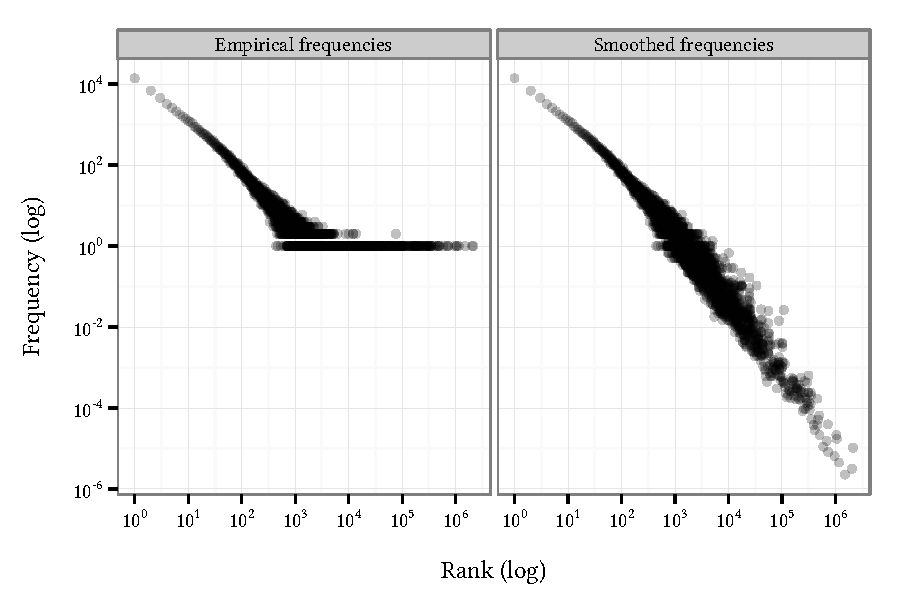
\includegraphics{zr.pdf}
\caption{The left panel shows the empirical word frequencies from the SUBTLEX-US frequency norms \citep{Brysbaert2009}. The right panel shows the same frequencies smoothed with the $Z_r$ transform.}
\label{subtlex}
\end{figure}


\bibliography{\jobname}
\bibliographystyle{pwpl}
\end{document}
